\chapter{Methods}
This chapter details the methods developed for semantic exploration, persistent 3D mapping, promptable object detection, and robust fusion strategies for multi-object search.

\section{System Overview}
\begin{itemize}
    \item Presentation of the overall architecture of the exploration, detection, mapping, and fusion pipeline.
    \item Description of data flow between exploration (frontier evaluation), detection (promptable models), and exploitation (persistent semantic mapping).
    \item Explanation of how exploration and mapping components interact to progressively build a semantic understanding of the environment.
\end{itemize}

\begin{figure}[h!]
    \centering
    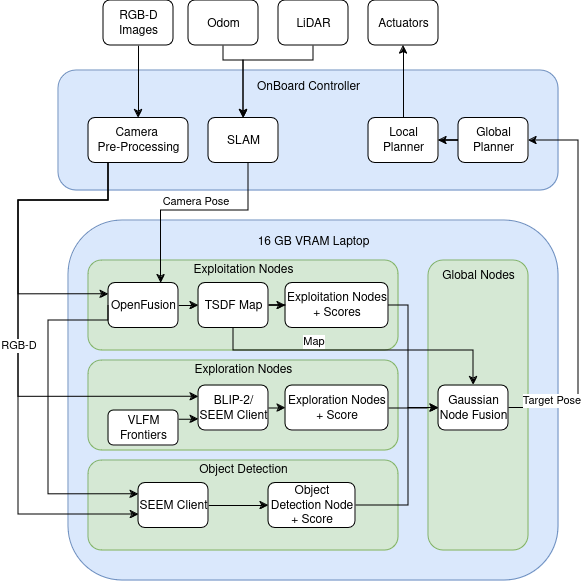
\includegraphics[width=\textwidth]{Images/03_methods/Master_Thesis_Overview.drawio.png}
    \caption{System architecture}
    \label{fig:system_overview}
\end{figure}

\section{Exploration Component: Semantic Frontier Mapping}
\subsection{Frontier Detection and Calculation}
\begin{itemize}
    \item Detection of frontiers on a 2D occupancy grid to identify candidate regions for exploration.
    \item Application of classical frontier-based exploration algorithms extended with semantic information.
\end{itemize}

\subsection{Value Map Generation using Vision-Language Models}
\begin{itemize}
    \item Computation of value maps by evaluating cosine similarity between multi-modal queries (text, image, audio) and scene observations.
    \item Use of promptable vision-language models (e.g., SEEM) to assign semantic relevance scores to each region.
    \item Dynamic update of value maps as new observations are integrated.
\end{itemize}

\subsection{Navigation to High-Value Frontiers}
\begin{itemize}
    \item Selection of the frontier with the highest semantic relevance score.
    \item Continuous re-evaluation of frontiers during exploration to adapt to changing scene semantics.
    \item Strategy for balancing exploration efficiency and semantic search goals.
\end{itemize}

\section{Exploitation Component: Persistent 3D Semantic Mapping}

\subsection{Global Map Construction with Open-Fusion}
\begin{itemize}
    \item Incremental creation of a global semantic point cloud map integrating RGB-D observations over time.
    \item Registration of observations using robot poses to maintain a consistent world representation.
    \item Association of semantic labels with 3D points based on query relevance scores.
\end{itemize}

\subsection{Semantic Clustering and Graph Node Generation}
\begin{itemize}
    \item Clustering of points with similar semantic labels to form object-level hypotheses.
    \item Construction of semantic graph nodes representing detected object instances with aggregated confidence scores.
    \item Maintenance of the semantic graph as a persistent memory for multi-object search tasks.
\end{itemize}

\section{Detection Component: Promptable Zero-Shot Models}
\begin{itemize}
    \item tbd
\end{itemize}

\section{Fusion Strategy: Confidence-Based Decision Making}
\begin{itemize}
    \item Formulation of a fusion strategy combining frontier-based semantic relevance with persistent 3D semantic mapping.
    \item Design of decision-making algorithms leveraging combined semantic information to robustly answer multi-object search queries.
\end{itemize}
